\documentclass[a4paper,11pt]{scrreprt}                       % default is A4 paper style and 11pt font size

%%%%% Author note for who reviews the code %%%%%%%
%Please use word warping for viewing the current LaTex source as it has been easier
%for me to write on a smaller screen. Apologiez for the long lines.
%Also, for anyone concerned, comments left here may come from the original authors of the template
%but otherwise the thesis' content is of my own contribution
%%%%%%%%%%%%%%%%%%%%%%%%%%%%%%%%%%%%%%%%%%%%%%%%%%%


%%%%%%%%%%%% version history %%%%%%%%%%%%%%%%%%%%%%%%%%%%%%%%%%%
%27.05.2021: updates about layout/plagiarism from Monica Patrascu, Bogdan Dumitrescu
%25.04.2020:  modified the lst definitions (monospaced, gray); localized versions (romanian) for the \autoref command; updated the romanian.lbx file
%26.03.2017:    corrections for the latex source-code: diacritics issues; corrected the glossaries and added listings packages; added fontspec (only works with xelatex/lualatex !!!)
%2014:          put in latex version + some small additions - Florin Stoican
%2013:          content from Dan Stefanoiu
%%%%%%%%%%%%%%%%%%%%%%%%%%%%%%%%%%%%%%%%%%%%%%%%%%%%%%%%%%%%%%%%%%%%%%%%%


%%%%%%%%%%%% macros for various paths %%%%%%%%%%%%%%%%%%%%%%%%%%%%%%%%%%%
\def \cls {./cls} 																					 % path to common latex files (change for your own relative/absolute path)
\def \pics {./pics}      																		 % path to pics files (change for your own relative/absolute path)
\def \chapters {./chapters}      														 % path to chapter files (change for your own relative/absolute path)
\def \code {./code}      													        	 % path to source code files (change for your own relative/absolute path)

% you don't have to use them but it's nicer this way
%%%%%%%%%%%%%%%%%%%%%%%%%%%%%%%%%%%%%%%%%%%%%%%%%%%%%%%%%%%%%%%%%%%%%%%%%

% language={english/romanian} selects between the languages used in the manusript (changes, e.g., the name of the chapter)
% type={bachelor/master/phd} selects between the type of manusript (changes, e.g., the titlepage make-up)
\usepackage[language=english,type=bachelor]{\cls/standard} % introduces useful packages and commands(CHANGE ONLY IF YOU KNOW WHAT YOU'RE DOING)
\addbibresource{\cls/bib.bib}																% bib resource (using biblatex package, for complex stuff use the biber backend instead of bibtex
\newglossaryentry{H-bridge}
{
    name=H-bridge,
    description={is a dedicated electronic circuit that switches the direction of current flow to a load, containing 4 switching elements, usually transistors, placed in a H shape}
}
\newglossaryentry{Kelvin connection}
{
    name=Kelvin connection,
    description={, also known as 4-wire sensing, is a circuit construction consisting of 4 connections across a circuit segment used in measuring low resistances; it is usually used in current measuring}
}

\newacronym{pwm}{PWM}{Pulse Width Modulation}
\newacronym{dc}{DC}{Direct Current}
\newacronym{ac}{AC}{Alternating Current}
\newacronym{pid}{PID}{Proportional-Integral-Derivative}
\newacronym[longplural={General Purpose Input/Output}]{gpio}{GPIO}{General Purpose Input/Output}
\newacronym{adc}{ADC}{Analog to Digital Converter}        																	% put here all your glossary terms; only the ones actually used will appear in the glossary list of the manuscript

\begin{document}

%%%%%%%%%%%%%%%%%%%%%%% frontmatter %%%%%%%%%%%%%%%%%%%%%%%%%%%%%%%%%%%%%
\pagenumbering{roman}																				% default numbering for the frontmatter is roman

\title{Discontinuous Current Conduction Mode in Solar Energy Production}					    % title of your manuscript
\author{Bontaș Cezar-Octavian}																				% author name
\advisor{Petrescu Cătălin-Dumitru}																			    % advisor name

\maketitle

% show table of contents, figures, tables and algorithms

\tableofcontents
\printnoidxglossaries																				% \printglossaries works only if the makeindex has the correct arguments
\listoffigures
\addcontentsline{toc}{chapter}{\listfigurename}
\listoftables
\addcontentsline{toc}{chapter}{\listtablename}
%\listofalgorithmes
%\addcontentsline{toc}{chapter}{\listalgorithmcfname}

\clearpage

%%%%%%%%%%%%%%%%%%%%%%% mainmatter %%%%%%%%%%%%%%%%%%%%%%%%%%%%%%%%%%%%%%
\pagenumbering{arabic}																			% default numbering for the mainmatter is arabic

% here is the text of you manuscript; you can put it directly here but it is better to include files (the main file will be more compact)
\chapter{Introduction}
\label{chap:introduction}
\chapter{Theoretical Aspects}
\label{chap:theoretical}

\myLettrine{S}{olar} power plants include multiple stages of converting the energy captured into varying voltage ranges and forms, either \gls{dc} or \gls{ac}, depending on the application that is used.
In general, these systems are integrated into the electrical grid infrastructure or used as power generators in the context of battery recharging or standalone operation in medium-sized industrial applications where the reliability on the traditional power infrastructures is rather poor. \cite{al2022photovoltaic}
\gls{pv} cells act as a \gls{dc} power source, but by themselves are insufficient for most practical applications, as they have to be connected in what is commonly known as solar panels, thus having different characteristics based on how these cells have been linked.
This usually leads to issues where the working characteristics of these panels have to be identified and mathematically modelled for efficient power conversion. \cite{al2022photovoltaic}
Additionally, the power output provided by these cells are affected by a multitude of external and internal factors, including, but not limited to:

\begin{itemize}
    \item Weather conditions, like rain, temperature and cloud coverage;
    \item Geographical positioning, as it reflects the maximum power available through solar irradiance;
    \item Cell degradation through aging of the internal p-n junction, thermal expansion and contraction, damaged induced by the elements (hailstone, winds carrying sand).
\end{itemize}

Thus, the power converted by these panels can vary drastically, and this variance in the input voltage provided by this source has to be accounted for when powering any load connected to the system.
A rough schematic of such system is included in \figref{fig:pvsystem}:

\begin{figure}[!ht]
    \begin{center}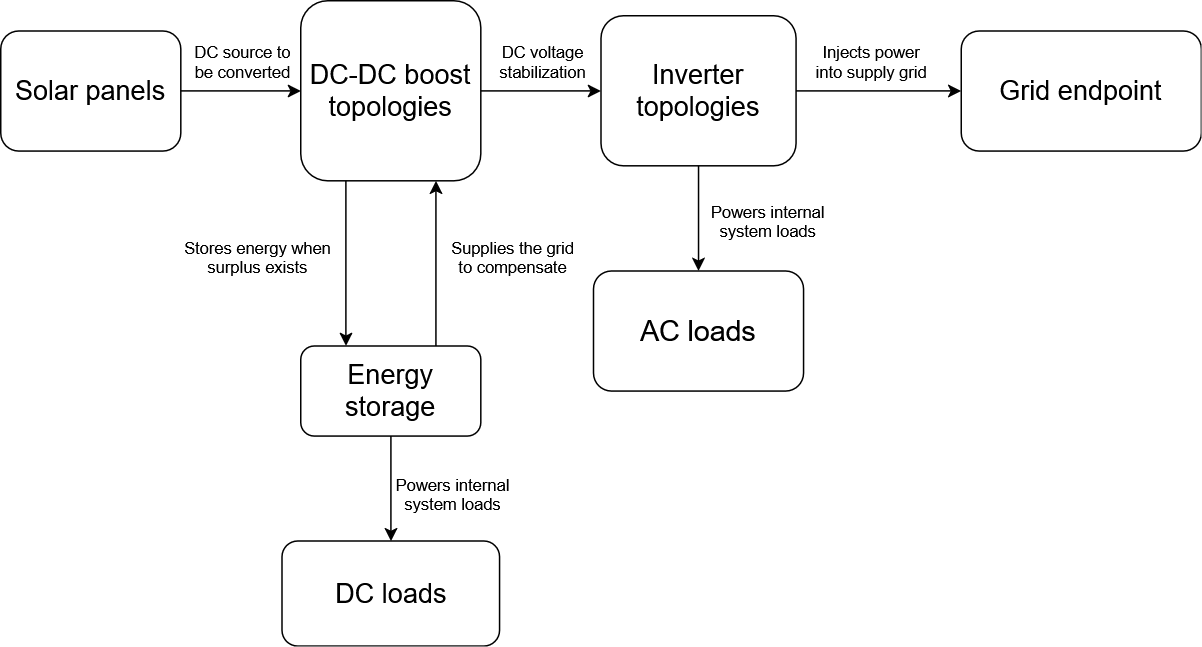
\includegraphics[width=\singlelongfigure]{\pics/models/pvsystem}\end{center}
    \caption{A typical configuration of a PV plant connected to a microgrid}
    \label{fig:pvsystem}
\end{figure}

As the paper focuses on inverter topologies, we assume the other system components behave within normal parameters and are not affected by significant defects.
The following sections will contain details about the chosen strategies for \gls{dc}-\gls{ac} conversion, topology used to implement this and the mathematical model of the circuit.

\section{The Anatomy of the Inverter System}
\label{sec:invsys}

\begin{figure}[!ht]
    \begin{center}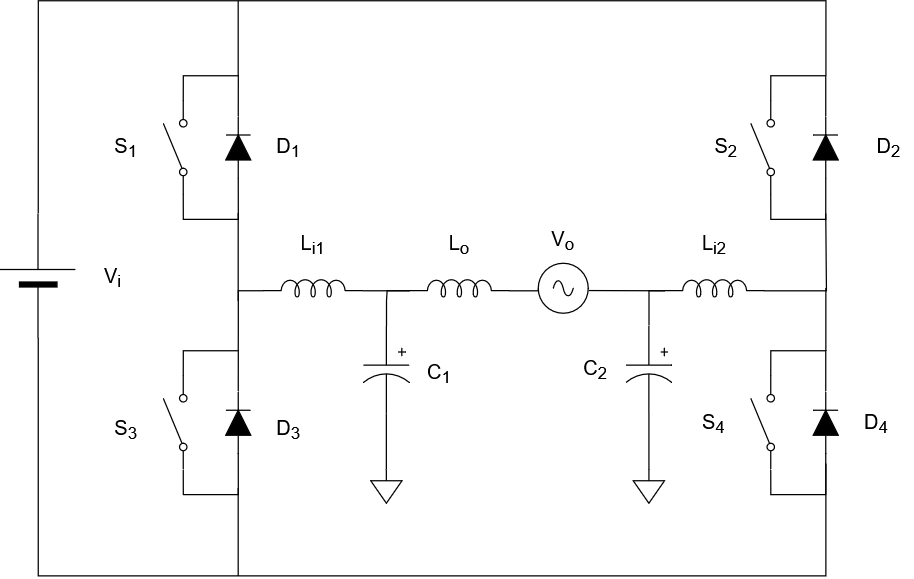
\includegraphics[width=\singlelongfigure]{\pics/models/hbridge}\end{center}
    \caption{The typical H-bridge structure with an LCL filter added at output}
    \label{fig:hbridge}
\end{figure}

Converting \gls{ac} current to \gls{dc} usually involves a simple diode rectifier, which is a passive circuit containing 4 diodes, meaning there isn't much to optimize in terms of electronic control besides physical construction.
However, the effort to do the opposite is considerably greater due to the fact that there is no circuit using only passive components that can modulate the voltage into a controlled sine wave.

\begin{table}[ht!]
\begin{tabular}{cccc}
\hline
State number & State description & Output voltage & Conducting components\\ 
 & & & for $i_o > 0$ \& $i_o < 0$ \\
\hline
1 & $S_1$ and $S_3$ open, $S_2$ and $S_4$ closed & $\frac{v_o}{2}$ & $S_1, S_3$ ; $D_1, D_3$\\
2 & $S_2$ and $S_4$ open, $S_1$ and $S_3$ closed & $-\frac{v_o}{2}$ & $S_2, S_4$ ; $D_2, D_4$\\
3 & $S_1$ and $S_2$ open, $S_3$ and $S_4$ closed & $0$ (short-circuit) & (not valid)\\
4 & $S_1$ and $S_2$ closed, $S_3$ and $S_4$ open & $0$ (short-circuit) & (not valid)\\
5 & $S_1$, $S_2$, $S_3$ and $S_4$ closed & $0$ (undefined) & $0$\\
\hline
\end{tabular}
\centering
\caption{All H-bridge states, with power outputs defined}
\label{tab:switchfunc}
\end{table}

The classic topology used for \gls{ac} power conversion is created using 4 switches in a formation known as a \gls{H-bridge} (example showcased in \figref{fig:hbridge}), with each half connected to one end of the load through a filter. \cite{rashid2013power}
Ideally, these switches are electrically controlled and don't possess any innate energy losses, however there are no such devices available with these characteristics.
The filter connected to each half bridge are designed to have 2 functions: they are energy storage devices that are used to create the sine wave injected into the grid, and they also reject high frequencies that are resulted from the residual energy consumption of the transistors' switching.
The principle behind converting the \gls{dc} current to \gls{ac} is by modulating the source voltage to match a carrier signal (in this case the load voltage) using a variable duty cycle \gls{pwm} signal that opens the transistors' gates.
These are switched alternatively to create both positive and negative voltages required for \gls{ac} forms, as shown in \tabref{tab:switchfunc}.

\section{Conduction Modes and Mathematical Model}
\label{sec:condmodes}

In any conversion switching circuit, there are two modes of conducting current through the filter inductors present in the topology, namely \gls{ccm} and \gls{dcm}.
These are related to how the current flowing through the circuit is stored into the inductor during any one switching cycle.
\gls{ccm} states that the current $i_{lx}$ should never drop to $0$ at any point in a cycle, whereas \gls{dcm} discharges the inductor completely until the time period elapses.
This comes with different advantages and disadvantages, such as requirements for inductor and capacitor sizes, presence of non-linear behaviour, conversion efficiency and maximum RMS current.
In the following subsections, there will be justifications provided for the usage of \gls{dcm} in the designed system.

\subsection{Justification for DCM Usage}
\label{subsec:justdcm}

Standard \gls{dc}-\gls{dc} and \gls{dc}-\gls{ac} conversion systems operate in \gls{ccm} due to its simplicity of writing a control algorithm for it as its behaviour is linear.
A simplified model of the system is presented in \figref{fig:ccmmodel}.

\begin{figure}[!ht]
    \begin{center}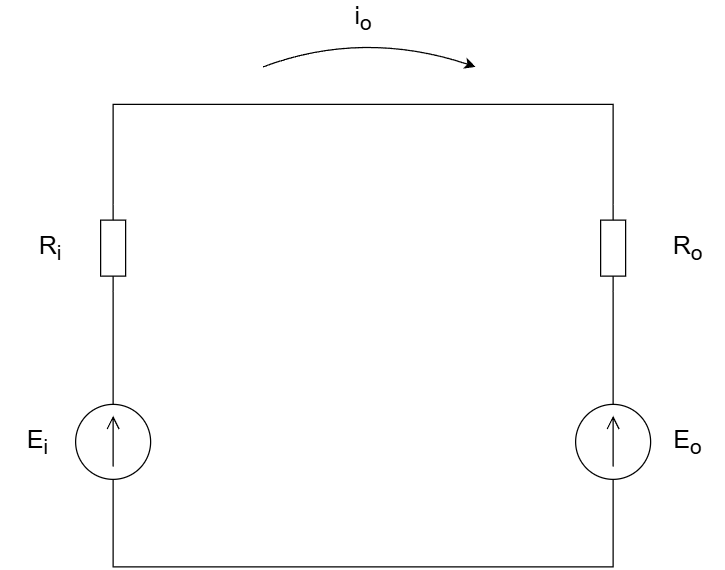
\includegraphics[width=\singlefigure]{\pics/models/ccmmodel}\end{center}
    \caption{Simplified model used for showcasing CCM}
    \label{fig:ccmmodel}
\end{figure}

The output voltage of the converter ($E_i$) depends on the duty cycle of the \gls{pwm} that drives the transistors as follows:
\begin{equation}
E_i = V_S \cdot q
\end{equation}
where $q$ is the duty cycle $[0, 1]$ of the \gls{pwm} signal and $V_S$ is the input source voltage that the system converts.
The output current $i_o$ would have the following form:
\begin{equation}
i_o = \frac{E_i - E_o}{R_i + R_o} = \frac{q \cdot V_S - E_o}{R_i + R_o}  
\end{equation}
Since the circuit is composed of 2 voltage sources placed in parallel and the internal resistances are ideally low in order to minimize energy losses, the output current is very sensitive to changes in the \gls{pwm} duty cycles.
As an example case, if we are to give values to each variable ($R_i = R_o = 1m\Omega, V_S = 12V, E_o = 3.6V$), $q$ would affect the output current as presented in \tabref{tab:ccmcur}.

\begin{table}[ht!]
\begin{center}
\begin{tabular}{|c|c|c|c|}
\hline
$i_o$ [A]&$E_i$ [V]&$q$ [\%]&PWM pulse length [ns]\\ \hline
0&3.600&30.000&120.000\\ \hline
50&3.700&30.833&123.333\\ \hline
-50&3.500&29.166&116.666\\ \hline
1&3.602&30.016&120.067\\ \hline
-1&3.598&29.983&119.933\\ \hline
0.1&3.6002&30.0016&120.0067\\ \hline
-0.1&3.5998&29.9983&119.9933\\ \hline
\end{tabular}
\end{center}
\caption{Experimental values provided using CCM control for the example system}
\label{tab:ccmcur}
\end{table}

It can be observed that the output current varies drastically even with small changes in the \gls{pwm} ratio, meaning that circuit control in this instance is a challenging task to achieve.
This would mean that many of the classic control methods used are inadequate unless the \gls{pwm} modulator can work with high resolutions.
Even if that is possible, as shown in \tabref{tab:ccmcur}, a small current change of $\pm 0.1A$ would require a change of $6.7ps$ in the \gls{pwm} pulse length, which is hard to achieve unless expensive hardware is utilized.
These kinds of frequencies cannot be achieved on microcontrollers, hardly on FPGAs, and are difficult to manage in circuit due to how susceptible to \gls{emi} the control signal is.

As mentioned previously at the beginning of \secref{sec:condmodes}, \gls{dcm} assumes that the energy stored in the filter inductor is fully discharged to the load at the end of each switching cycle.
This means that the system acts as a constant power source rather than a constant voltage source, which would mitigate the effects described previously.

\subsection{Explaining Converter Operation Under CCM vs DCM}
\label{subsec:ccmvsdcm}

\begin{figure}[!ht]
    \begin{center}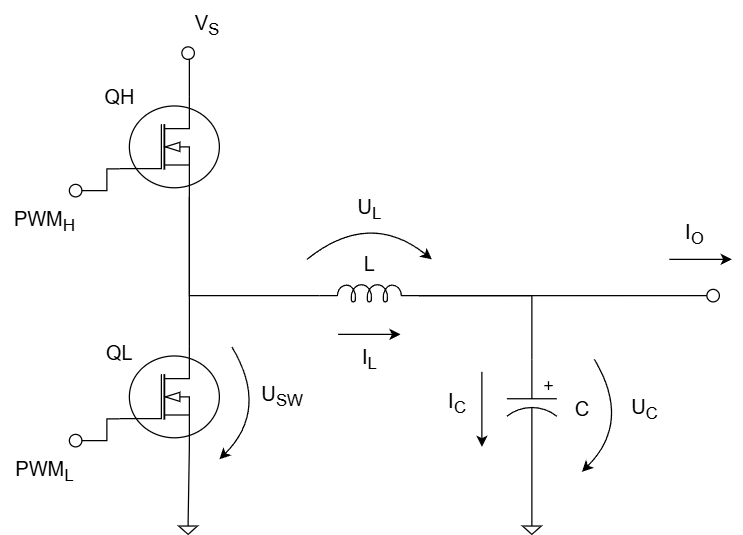
\includegraphics[width=\doublefigure]{\pics/models/bridgelc}\end{center}
    \caption{Simplified model of a half-bridge converter}
    \label{fig:bridgelc}
\end{figure}

\gls{H-bridge} topologies used in current conversions can be split up into two symmetrical half-bridge circuits as the control inputs are mirrored.
This part focuses on how each branch stores the converted input current ($I_o$) using the filter inductor on an LC filter.
A simplified version of such structure is presented in \figref{fig:bridgelc}.

In most cases where \gls{ccm} is used, the command signals $PWM_L$ and $PWM_H$ are generated similar to \figref{fig:pwmccm}, where $T_o$ is the constant period of the \gls{pwm} signal and $T_h$ is the pulse duration that controls the converter operation.
\begin{figure}[!ht]
    \begin{center}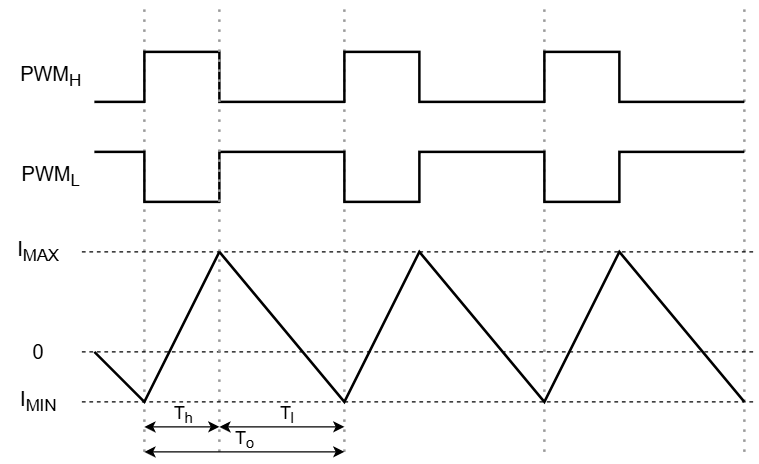
\includegraphics[width=\singlefigure]{\pics/models/pwmccm}\end{center}
    \caption{Current stored in the filter inductor under CCM}
    \label{fig:pwmccm}
\end{figure}

It can be observed that MOSFETs $QL$ and $QH$ (which is the most popular choice for small to medium voltage applications), are switched complementary.
Since MOSFETs allow current to pass in both directions when the conduction state is active, there are no restrictions  on the polarity of the current that passes through the inductor during switching period $T_o$.
Depending on the command signals $PWM_H$ and $PWM_L$, the converter can be found in one of these two states:
\begin{itemize}
    \item $PWM_H = 1$ and $PWM_L = 0$
    During this state, the switch node voltage $U_{SW} = V_S$ and the inductor changes according to:
    \begin{equation}
        \frac{dI_L}{dt} = \frac{U_L}{L} = \frac{U_{SW} - U_C}{L} = \frac{V_S - U_C}{L}
    \end{equation}
    The capacitor value is chosen large enough to assure a very small variation of its voltage during a switching period.
    As a result, the derivate of the inductor current is constant and has a positive value because $V_S > U_C$.
    This statement allows to approximate the inductor current as:
    \begin{equation}
        I_l(t) = I_{MIN} + \frac{dI_L}{dt} \cdot t = I_{MIN} + \frac{V_S - U_C}{L} \cdot t
    \end{equation}
    At the end of the $T_h$ time period where the converter transitions to the next state, the inductor current value will be as follows:
    \begin{equation}
        I_L(T_h) = I_{MIN} + \frac{V_S - U_C}{L} \cdot T_h = I_{MAX}
    \end{equation}
    
    \item $PWM_H = 0$ and $PWM_L = 1$
    During this stare, the switch node voltage $U_{SW} = 0$ and the inductor current changes according to:
    \begin{equation}
        \frac{dI_L}{dt} = \frac{U_L}{L} = \frac{U_{SW} - U_C}{L} = -\frac{U_C}{L}
    \end{equation}
    Assuming constant voltage across the capacitor, inductor current value can be approximated as:
    \begin{equation}
        I_L(t) = I_{MAX} + \frac{dI_L}{dt} \cdot (t - T_h) = I_{MAX} - \frac{U_C}{L} \cdot (t - T_h)
    \end{equation}
    At the end of the remaining time period $T_l$ where the next switching event will happen, the inductor current value will be:
    \begin{equation}
        I_L(T_h + T_l) = I_{MAX} - \frac{U_C}{L} \cdot T_l
    \end{equation}
\end{itemize}

In the steady state, $I_L(T_h + T_l) = I_{MIN}$ leads to:
\begin{equation}
    I_{MAX} - \frac{U_C}{L} \cdot T_l = I_{MIN}
\end{equation}
Replacing $I_{MAX}$ we obtain:
\begin{equation}
    I_{MIN} + \frac{V_S - U_C}{L} \cdot T_h - \frac{U_C}{L} \cdot T_l = I_{MIN}
\end{equation}
that gives the relation between voltages and switching time periods:
\begin{equation}
    \label{eq:ccmv2t}
    (V_S - U_C) \cdot T_h = U_C \cdot T_l
\end{equation}
If we consider that $T_l = T_o - T_h$, equation \eqref{eq:ccmv2t} becomes:
\begin{equation}
    (V_S - U_C) \cdot T_h = U_C \cdot (T_o - T_h)
\end{equation}
which in turn can be written as:
\begin{equation}
    \label{eq:finalccm}
    U_C = V_S \cdot \frac{T_h}{T_o} = q \cdot V_S
\end{equation}
Equation \eqref{eq:finalccm} shows that the half-bridge converter behaves as a controlled voltage source, and as presented in \subsecref{subsec:justdcm}, it makes current control substantially difficult.

To operate the converter in \gls{dcm} it is necessary to modify the gate control signals applied to the MOSFETs as follows:
\begin{itemize}
    \item if $I_o > 0$, the \gls{pwm} signal is applied only on the high-side transistor (QH)
    \item if $I_o < 0$, the \gls{pwm} signal is applied only on the low-side transistor (QL)
\end{itemize}
In \gls{dcm}, the inductor current is 0 at the beginning of each switching period and reaches the value of 0 before the end of switching period $T_o$.
If the \gls{pwm} signal is applied to the high-side transistor, the inductor current will have the evolution shown in \figref{fig:pwmdcm1}.

\begin{figure}[!ht]
    \begin{center}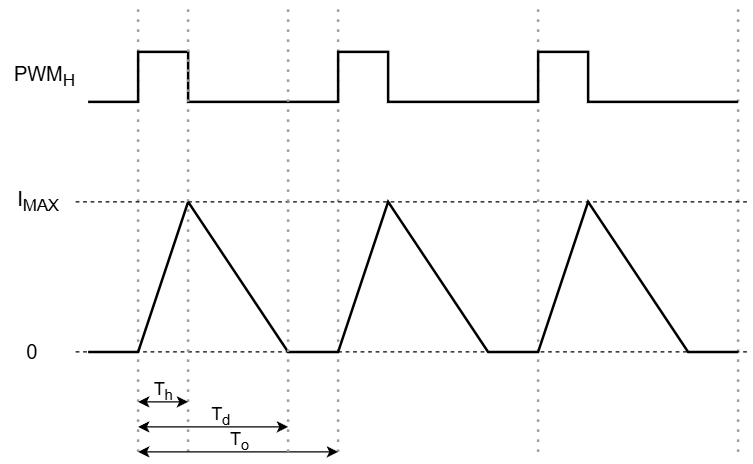
\includegraphics[width=\singlefigure]{\pics/models/pwmdcm1}\end{center}
    \caption{Current stored in the filter inductor under DCM using the high-side transistor}
    \label{fig:pwmdcm1}
\end{figure}

During the $T_h$ period, the switch node voltage $U_{SW} = V_S$ and the inductor current changes according to:
\begin{equation}
    I_L(t) = \frac{dI_L}{dt} \cdot t = \frac{V_S - U_C}{L} \cdot t
\end{equation}
At the end of the $T_h$ interval, the inductor current value will be:
\begin{equation}
    I_L(T_h) = \frac{V_S - U_C}{L} \cdot T_h = I_{MAX}
\end{equation}
After the MOSFET is turned off, the inductor current will flow through the internal body of the low-side transistor and the switch node voltage $U_{SW} = 0$ (assuming an ideal diode).
As a result, the inductor current will change according to:
\begin{equation}
    \begin{split}
        I_L(t) &= I_{MAX} + \frac{dI_L}{dt} \cdot(t - T_h)  \\
        &= I_{MAX} - \frac{U_C}{L} \cdot (t - T_h) \\
        &= \frac{V_S - U_C}{L} \cdot T_h - \frac{U_C}{L} \cdot (t - T_h)
    \end{split}
\end{equation}
When both time periods $T_h$ and $T_d$ ($t = T_h + T_d$) have elapsed, the inductor current becomes 0, which in turn would mean:
\begin{equation}
    \label{eq:lcurt}
    I_L(T_h + T_d) = \frac{V_S - U_C}{L} \cdot T_h - \frac{U_C}{L} \cdot [(T_h + T_d) - T_h] = 0
\end{equation}
From equation \eqref{eq:lcurt}, inductor discharge time $T_d$ can be written as:
\begin{equation}
    T_d = T_h \cdot \frac{V_S - U_C}{U_C}
\end{equation}
After this moment, the internal body diode will prevent the current through the inductor to drop at a negative value, therefore remaining at 0.

In the steady state, the output current $I_o$ is equal to the average value of the inductor current which is:
\begin{equation}
    \begin{split}
        I_o = (I_L)_{med} &= \frac{I_{MAX}}{2} \cdot \frac{T_h + T_d}{T_o} \\
        &= \left(\frac{V_S - U_C}{2 \cdot L} \cdot T_h\right) \cdot \frac{T_h}{T_o} \cdot \left(1 + \frac{V_S - U_C}{U_C}\right) \\
        &= \frac{V_S}{2 \cdot L \cdot T_o} \cdot \frac{V_S - U_C}{U_C} \cdot T_h^2
    \end{split}
\end{equation}

The condition for operating in \gls{dcm} is that $T_h + T_d < T_o$ that leads to:
\begin{equation}
    T_h + T_h \frac{V_S - U_C}{U_C} < T_o
\end{equation}
that imposes a maximum value for the transistor conduction period $T_h$:
\begin{equation}
    T_h < T_o \frac{U_C}{V_S}
\end{equation}
This condition limits the value of the output current to keep the converter to operate in \gls{dcm}:
\begin{equation}
    I_o < \frac{(V_S - U_C) \cdot U_C \cdot T_o}{2 \cdot L \cdot V_S} = \frac{V_S \cdot T_o}{2 \cdot L} \cdot \frac{U_C}{V_S} \cdot \left(1 - \frac{U_C}{V_S}\right)
\end{equation}
To ensure that the converter remains in \gls{dcm} regardless of the voltage across the capacitor, inductor value must be chosen as:
\begin{equation}
    L < L_{max} = \frac{V_S \cdot T_o}{2 \cdot I_o^{max}} \cdot min\left\{\frac{U_C^{min}}{V_S} \cdot \left(1 - \frac{U_C^{min}}{V_S}\right), \frac{U_C^{max}}{V_S} \cdot \left(1 - \frac{U_C^{max}}{V_S}\right)\right\}
\end{equation}

If the \gls{pwm} signal is applied to the low-side transistor, the inductor current will have the evolution described in \figref{fig:pwmdcm2}.

\begin{figure}[!ht]
    \begin{center}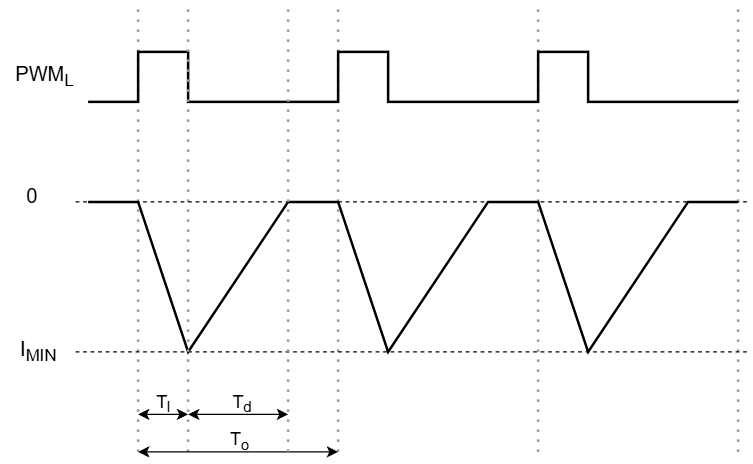
\includegraphics[width=\singlefigure]{\pics/models/pwmdcm2}\end{center}
    \caption{Current consumed by the filter inductor under DCM using the low-side transistor}
    \label{fig:pwmdcm2}
\end{figure}

During the $T_l$ period, the switch node voltage $U_{SW} = 0$ and the inductor current changes according to:
\begin{equation}
    I_L(t) = \frac{dI_L}{dt} \cdot t = -\frac{U_C}{L} \cdot
\end{equation}
At the end of the $T_l$ interval, the inductor current value will be:
\begin{equation}
I_L(T_l) = -\frac{U_C}{L} \cdot T_l = I_{MIN}
\end{equation}
After the MOSFET transistor is turned off, the inductor current will flow through the internal body diode of the high-side transistor and the switch node voltage $U_{SW}$ will become $V_S$ (assuming it is an ideal diode).
As a result, the inductor current will change according to:
\begin{equation}
    \begin{split}
        I_L(t) &= I_{MIN} + \frac{dI_L}{dt} \cdot (t - T_l) \\
        &= I_{MIN} + \frac{V_S - U_C}{L} \cdot (t - T_L) \\
        &= -\frac{U_C}{L} \cdot T_l + \frac{V_S - U_C}{L} \cdot (t - T_l)
    \end{split}
\end{equation}
When both time periods $T_h$ and $T_d$ ($t = T_h + T_d$) have elapsed, the inductor current becomes 0, which in turn would mean:
\begin{equation}
    I_L(T_l + T_d) = -\frac{U_C}{L} \cdot T_l + \frac{V_S - U_C}{L} \cdot [(T_l + T_d) - T_l] = 0
\end{equation}
From this equation, inductor discharge time $T_d$ can be obtained as:
\begin{equation}
    T_d = T_l \frac{U_C}{V_S - U_C}
\end{equation}
After $T_d$ elapses, the internal body diode will prevent the current through the inductor to raise beyond 0, therefore its value will remain zero.

In the steady state, the output current $I_o$ is equal to the average value of the inductor current which can be written as:
\begin{equation}
    \begin{split}
        I_o = (I_L)_{med} &= \frac{I_{MAX}}{2} \cdot \frac{T_l + T_d}{T_o} \\
        &= \left(-\frac{U_C}{2 \cdot L} \cdot T_l\right) \cdot \frac{T_l}{T_o} \cdot \left(1 + \frac{U_C}{V_S - U_C}\right) \\
        &= \frac{V_S}{2 \cdot L \cdot T_o} \cdot \frac{U_C}{V_S - U_C} \cdot T_l^2
    \end{split}
\end{equation}
In this case, the condition for operating in \gls{dcm} is $T_l + T_d < T_o$, which leads to:
\begin{equation}
    T_l + T_l \frac{U_C}{V_S - U_C} < T_O
\end{equation}
that imposes a maximum value for transistor conduction time period $T_l$:
\begin{equation}
    T_l < T_o \frac{V_S - U_C}{V_S}
\end{equation}
This condition leads to a maximum value for the negative output current to keep the converter operating in \gls{dcm}:
\begin{equation}
    I_o > -\frac{(V_S - U_C) \cdot U_C \cdot T_o}{2 \cdot L \cdot V_S} = -\frac{V_S \cdot T_o}{2 \cdot L} \cdot \frac{U_C}{V_S} \cdot \left(1 - \frac{U_C}{V_S}\right) 
\end{equation}
which has the same absolute value as the maximum current output when conducting the high-side transistor.
If the output current must be in the range of $[-I_o^{max}, +I_o^{max}]$, the condition that assures the operation in \gls{dcm} is:
\begin{equation}
    L < L_{max} = \frac{V_S \cdot T_o}{2 \cdot I_o^{max}} \cdot min\left\{\frac{U_C^{min}}{V_S} \cdot \left(1 - \frac{U_C^{min}}{V_S}\right), \frac{U_C^{max}}{V_S} \cdot \left(1 - \frac{U_C^{max}}{V_S}\right)\right\}
\end{equation}
\chapter{Proposed Model}
\label{chap:model}
\chapter{Practical Aspects}
\label{chap:practical}

\myLettrine{G}{iven} the previously described topology and ideal model of the proposed solar inverter system in \chapref{chap:solution}, there is a need to implement this solution into a physical circuit in order to effectively determine the efficiency of this implementation.
This step is achieved by creating the design of a dedicated \gls{pcb} that contains the \gls{H-bridge}, passive filtering circuitry and logic control sections, combined with the \gls{pid} controller and current measurements implemented at the software level.
The solution I am proposing in the following sections have been made with these energy targets in mind:
\begin{itemize}
    \item Input voltage ($V_{in}$) is $24V$ \gls{dc};
    \item Output voltage ($V_{out}$) is $12V$ \gls{ac};
    \item RMS current converted ($I_{RMS}$) is around $2.5A$;
\end{itemize}
thus converting the equivalent of $30W$.
These characteristics are only ideal, as there are no perfect components and energy losses are unavoidable, however for the scope of this thesis, this should be enough to demonstrate the efficiency of the chosen topology.

\section{Hardware Implementation}
\label{sec:hwimp}

The process of designing the electronic device is split into choosing the main components (microcontroller, switching elements, current measuring resistor, operational and instrumentation amplifiers, passive components specific to the filtering), drawing the schematic of the board, simulating the design and doing the \gls{pcb} layout.
This has been done using KiCad, a free and open source CAD program that has more than enough features to aid in the development of the \gls{pcb} in question.

\subsection{Component Selection}
\label{subsec:compsel}

Arguably the most important section of the whole circuit is the \gls{H-bridge}, which allows for the formation of the current sine wave present in any \gls{ac} signal.
In most common instances, the bridge is composed of 4 transistors, either MOSFETs or IGBTs, that act as electronically commanded switches to the inverter system. On this prototype, size and cost are a priority over efficiency and maximum power rating, as long as these components can achieve the proposed target.
For this, I have chosen 2 IFX007Ts, which are \gls{ic}s containing a half-bridge and gate drivers, used primarily for motor control, but these can also be used in power conversion applications.
Since they can withstand up to $50A$ of current flowing through the drain and operate up to $40V$, these components satisfy the required targets.

Passive components chosen for the LCL filter are crucial in order to block residual high frequencies caused by the \gls{pwm} switching and any other external sources of noise\cite{reznik2013lcl, systematiclcl2015}.
Criteria for choosing these consist of low ESR values, which in turn would mean higher power conversion efficiency, tolerance values of the main characteristic of that component, maximum saturation current for the inductors and low ripple current for the capacitors.
Hybrid aluminum polymer capacitors exhibit such good values, and for inductors, specialized flexible transformer have been used, as the windings can be independently connected in serial and parallel configurations. This achieves different turn ratios, inductance and current-carrying capabilities.

\begin{figure}[!ht]
    \begin{center}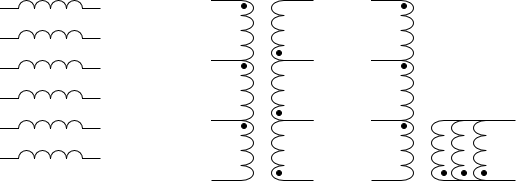
\includegraphics[width=\singlefigure]{\pics/schematics/transformerconfigs}\end{center}
    \caption{WE-FLEX transformer overview and example configurations}
    \label{fig:transf}
\end{figure}

The main take from \figref{fig:transf} is the following: the flexible transformer chosen can be thought of as 6 independent coils that can be connected in any way (as long as polarities are respected, market with a dot).
Knowing the base inductance per turn ($L_{base}$) is $12\mu H$ and the base current is $1.7A$, coils put in parallel multiply the base current rating, and windings put in series increase the inductance of the primary/secondary couple in accordance to this equation:
\begin{equation}
    \label{eq:Lwindings}
    L_{res}=L_{base} \cdot N_{sw}^2
\end{equation}
where $N_{sw}$ is the number of windings in series.
For the given examples, the middle configuration turns into a 1:1 ratio, $108\mu H$ transformer that can carry $1.7A$ of RMS current, and the right configuration is a 3:1 ratio transformer that has the same values on the primary as the former configuration, but the secondary can carry $5.1A$ with inductance $12\mu H$.

The feedback loop needs some way to have currents and voltages measured in order to calculate the next command to be given, thus a special current sense resistor is utilized in the circuitry.
This resistor has a low resistance value (usually under $1\Omega$), near 0\% tolerances and higher power ratings since they dissipate heat proportional to the current driven on the power traces, and it should not have its resistance drift with temperature changes.
Since we expect to deliver at least $2.5A$ RMS current through the \gls{pcb} traces, and to have minimal voltage drop across the resistor's terminals, I've chosen the WSLP2512R0100FEA, which is a $10m\Omega$, $\pm 1\%$ SMD resistor that can withstand $3W$ of power.
This is sufficient, as per Joule's first law:
\begin{equation}
    \label{eq:Joulefirstlaw}
    P = I^2 \cdot R
\end{equation}
it would result in a peak power dissipation of around $0.01\Omega \cdot (10A)^2 = 1W$, which is a third of the maximum power rating and a safe value to consistently maintain without damaging the component\cite{scherz2006practical}.

\begin{figure}[!ht]
    \begin{center}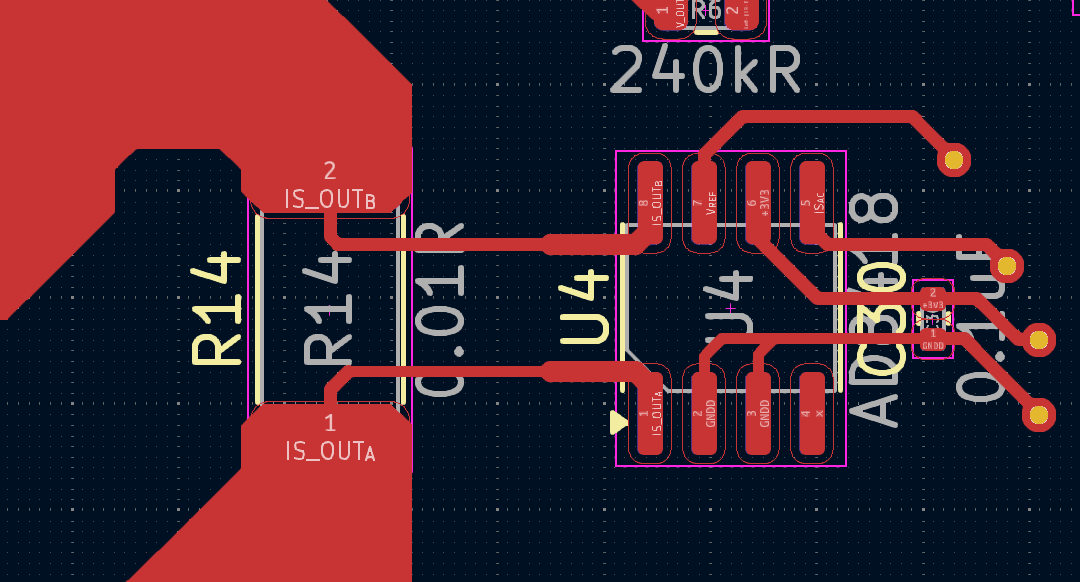
\includegraphics[width=\singlefigure]{\pics/schematics/kelvincon}\end{center}
    \caption{Example of Kelvin connections, voltage terminals come from inside the pads}
    \label{fig:kelvin}
\end{figure}

The voltage sensing terminals are then connected through \gls{Kelvin connection} (as shown in \figref{fig:kelvin}) to operational amplifiers and instrumentation amplifiers, like the MCP6001 and the AD8418 series respectively, used for amplifying the signal's gain and reject common-mode signals.
Current can't be directly measured, however the voltage drop on the shunt can be quantified, and since it is defined to be small in order to minimize losses, gain amplification needs to be done\cite{scherz2006practical}.
To calculate the source current, we can use Ohm's law:
\begin{equation}
    \label{eq:Ohmslaw}
    V = I \cdot R
\end{equation}
where the voltage is measured and resistance is already known.

All of these functions are tied to the microcontroller, that converts the values measured of the analog signals using the \gls{adc}s into numeric values, and these values are used as reference and system output in order to recalculate the \gls{pwm} duty cycles which modulates the carrier signal through the \gls{gpio}, or in this case, the converted \gls{ac} power source.
As discussed in \secref{sec:simrec} the period of the \gls{pwm} signal has been chosen to be of $20\mu s$, so any microcontroller which can output 50KHz signals and can calculate the next duty cycle in the meantime is fit for this project.
The choice of PSoC3M5 series has been mostly arbitrary, with the mention that ARM microcontrollers have been a popular choice in recent years as the CPU's architecture is easier to integrate into more complex SoCs.
Given the fact that it integrates 16 \gls{adc} channels, all digital pins have the capability of \gls{pwm} output, can operate at up to 180MHz and has numerous \gls{gpio} pins for additional expansion of functionality for debugging processes, it should be more than enough for this application.

\subsection{Electronic Circuit Overview}
\label{subsec:cirtdesc}

\begin{figure}[ht]
    \begin{center}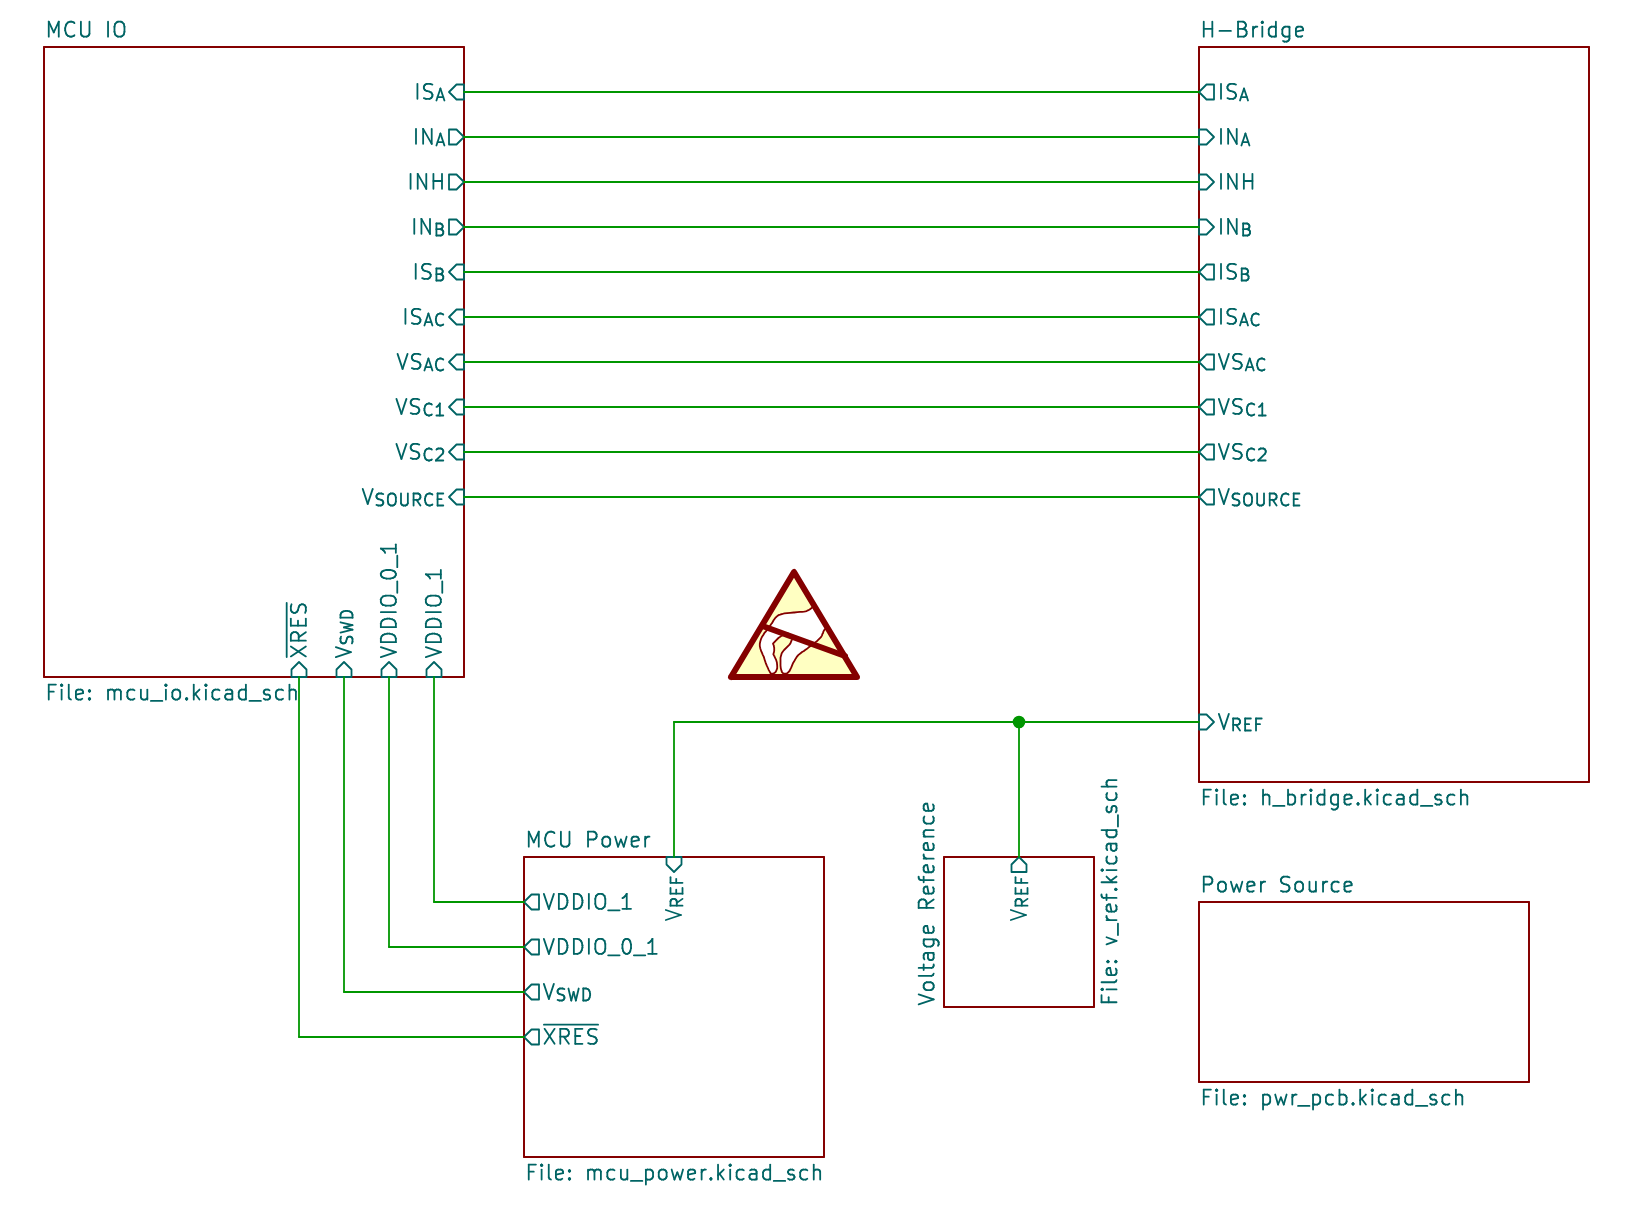
\includegraphics[width=10cm]{\pics/schematics/mainsch}\end{center}
    \caption{Schematic being split into functional blocks, with interconnects}
    \label{fig:mainsch}
\end{figure}

Once main component selection is done, the next step in designing the solution is to create the schematic of the circuit in order to describe how each of the parts will be connected together to form the power conversion topology, logic control and auxiliary power supply for the board to function.
It is important to note that in its description, the schematic representation is different from the layout, as the former shows at a functional level how each component is connected, while the latter contains the physical representation of these connections and other board properties such as layer definition and stack up and component placement.
To make the design easier to understand, the schematic has been split into multiple sections, as shown in \figref{fig:mainsch}.

The appropriately named \textit{H-Bridge} is responsible for the \gls{dc}-\gls{ac} conversion using the transistor bridge using 2 IFX007T as discussed in the previous subsection. The input current from the source, denoted by the connector $J1$ is passed to each half bridge \gls{ic}s, controlled using the signals $IN_{A}$, $IN_{B}$, and common inhibit signal $INH$.
$IN_{A}$ and $IN_{B}$ are the signals setting up bridge configuration; these should always have opposite values to prevent short-circuits.
$INH$ is the signal which modulated using \gls{pwm} would regulate the current conduction through its respective transformer connected to in series.
The output of each \gls{ic} is then passed through the LCL filter, which utilizes the transformers in 2 stages: the first has all of the windings connected in parallel ($T1$ and $T2$), which would form a $12\mu H$ inductor, while the second transformer ($T3$) is configured as a series of 3 groups of 2 parallel windings that results a $108\mu H$ value.

\begin{figure}[!ht]
    \begin{center}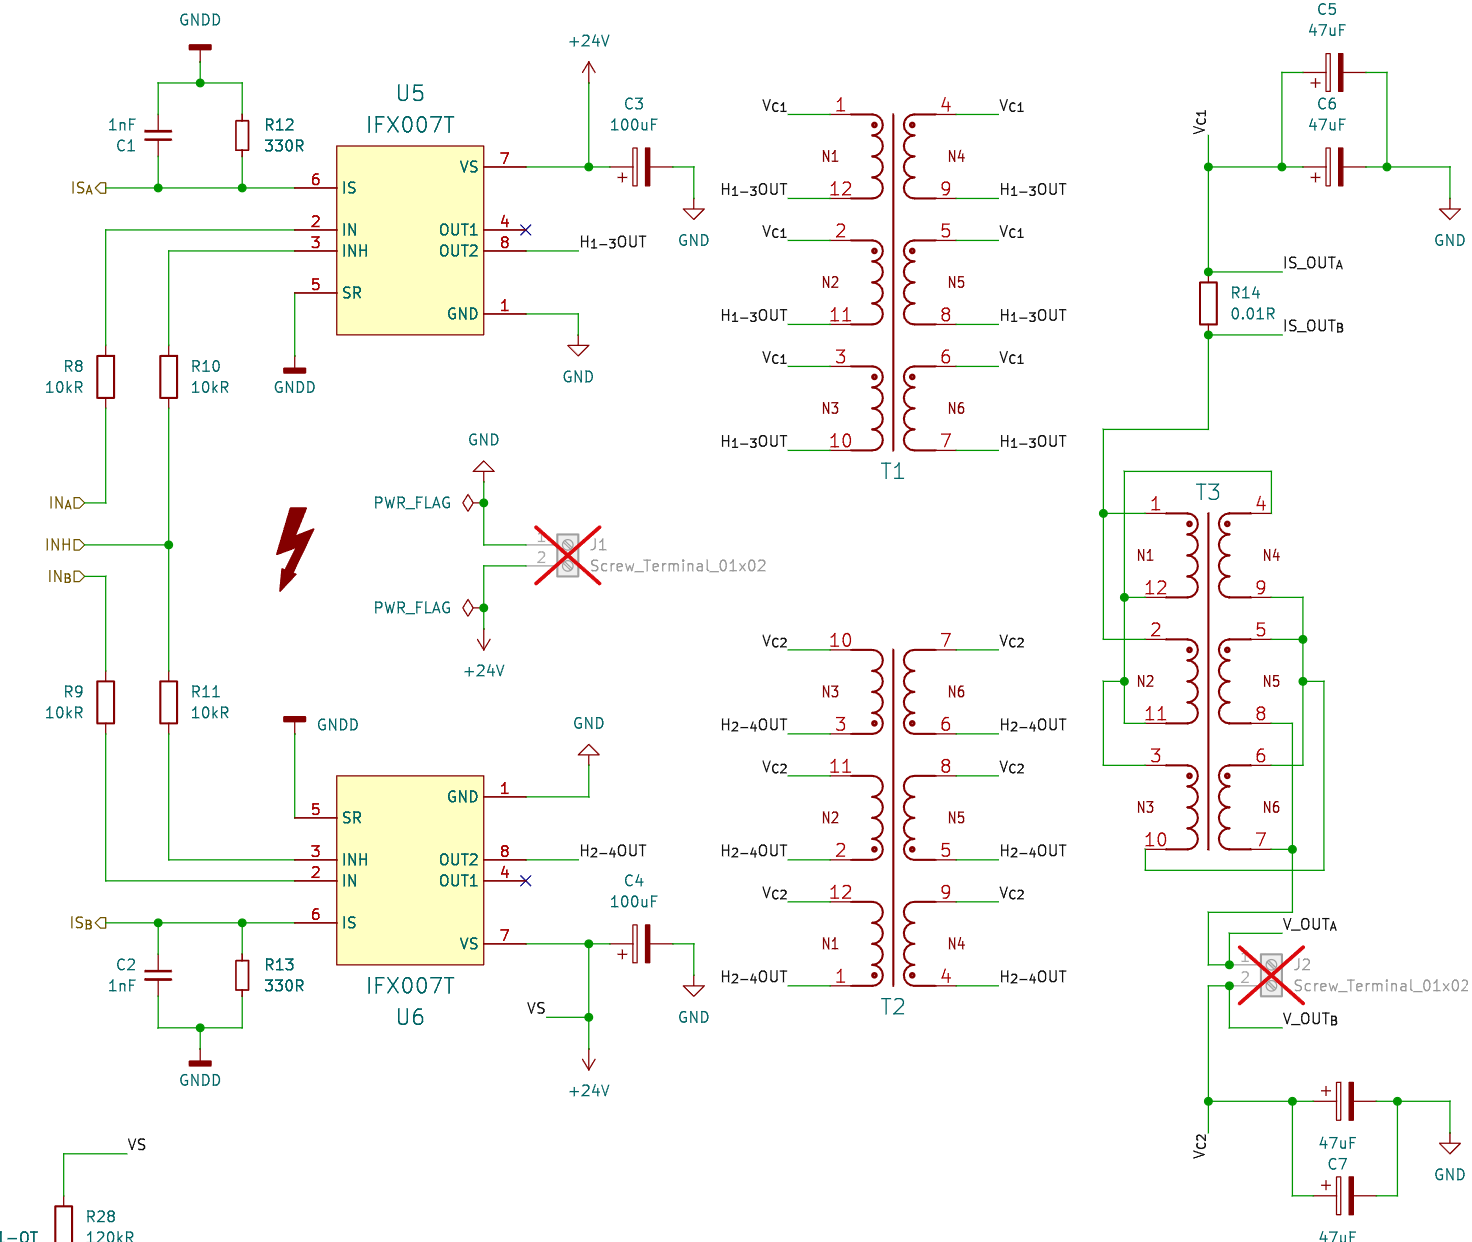
\includegraphics[width=\singlelongfigure]{\pics/schematics/hbridge}\end{center}
    \caption{Schematic of the implemented topology}
    \label{fig:hbridgesch}
\end{figure}

While the expected voltage that is injected into the grid through $J2$ should be 24V, to be sure that the feedback loop is correctly implemented, dedicated measurement circuitry is added on the board to know output voltage, output current that the board regulates through the $R12$ shunt, input source voltage (denoted through the $VS$ label), and voltages across both arms of the low-pass filter.

\begin{figure}[!ht]
    \begin{center}
        \subfloat[output voltage]{\label{fig:getvout}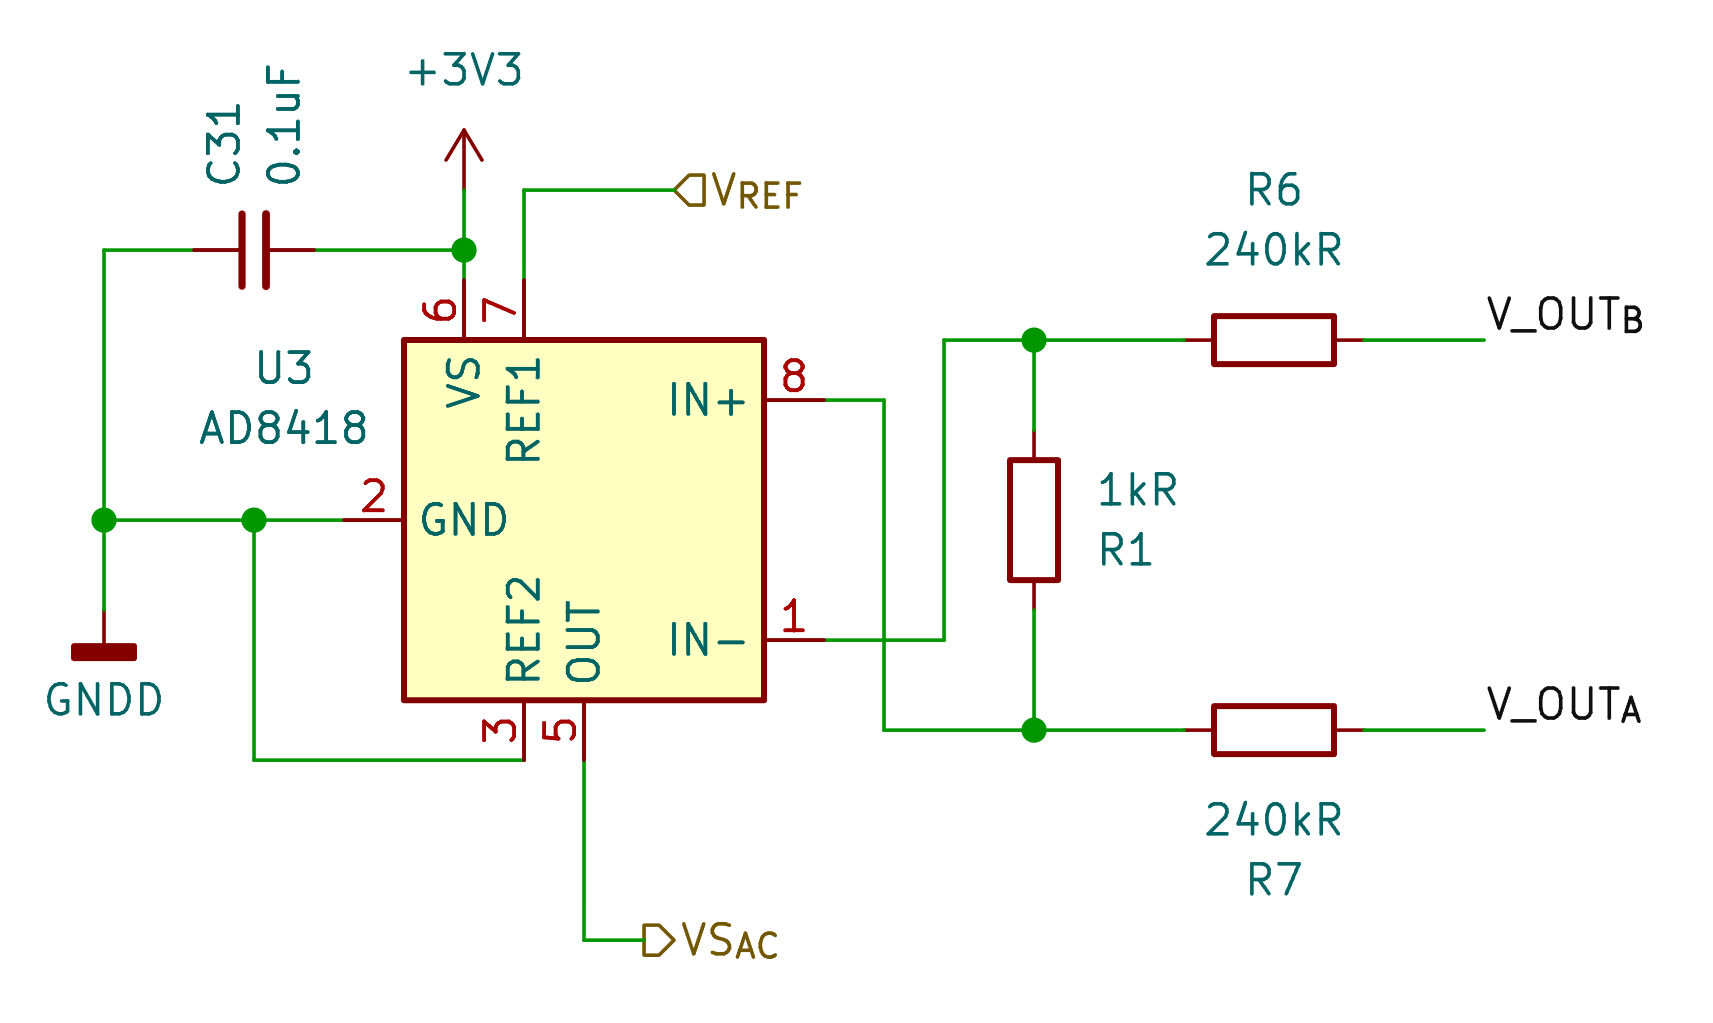
\includegraphics[width=\triplefigure]{\pics/schematics/voltageshunt}}
        \subfloat[output current]{\label{fig:getiout}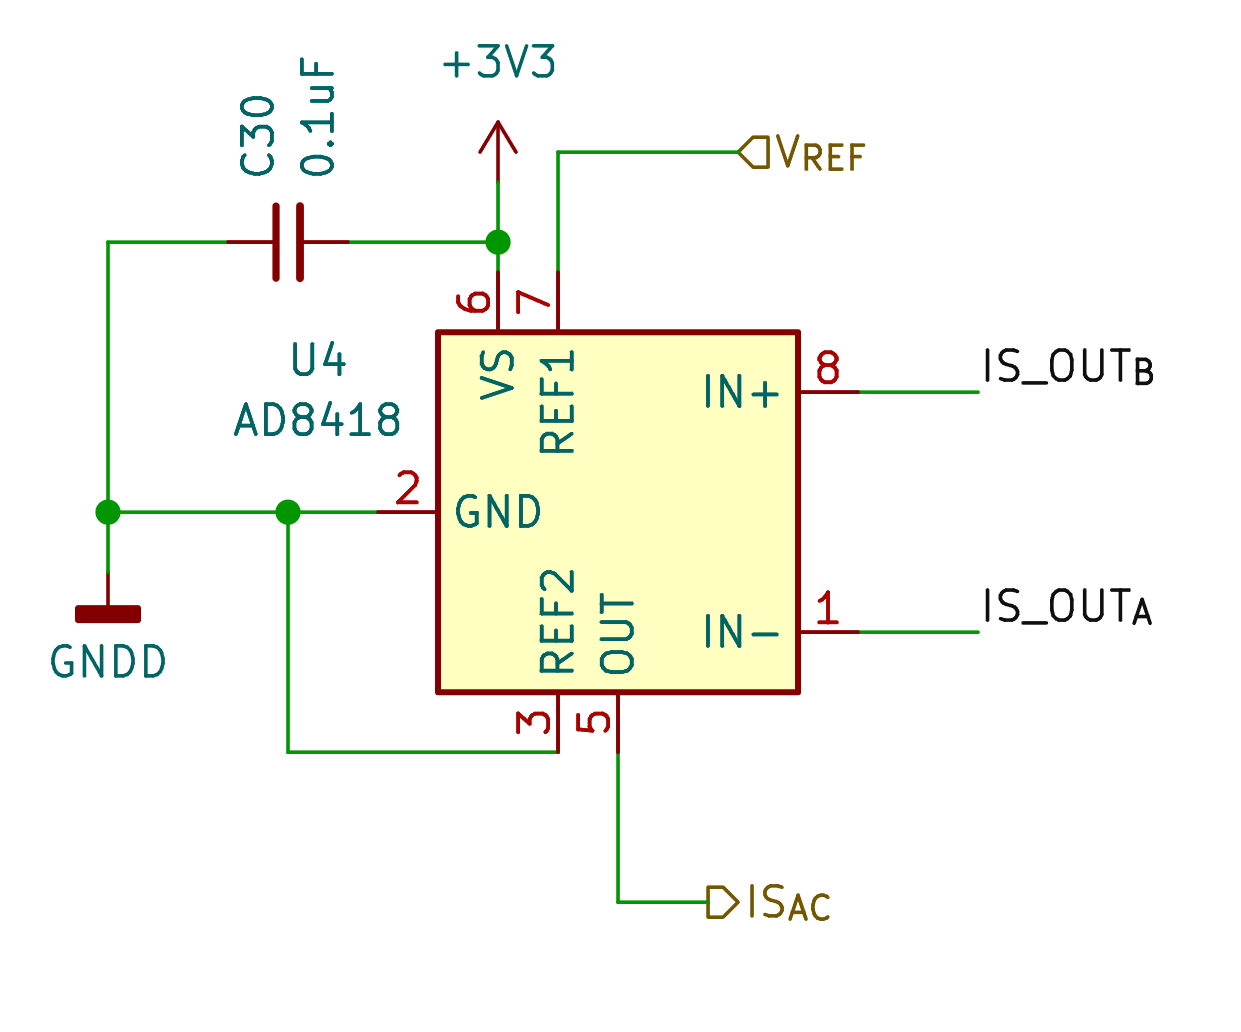
\includegraphics[width=\triplefigure]{\pics/schematics/currentshunt}}
        \subfloat[input voltage]{\label{fig:getvin}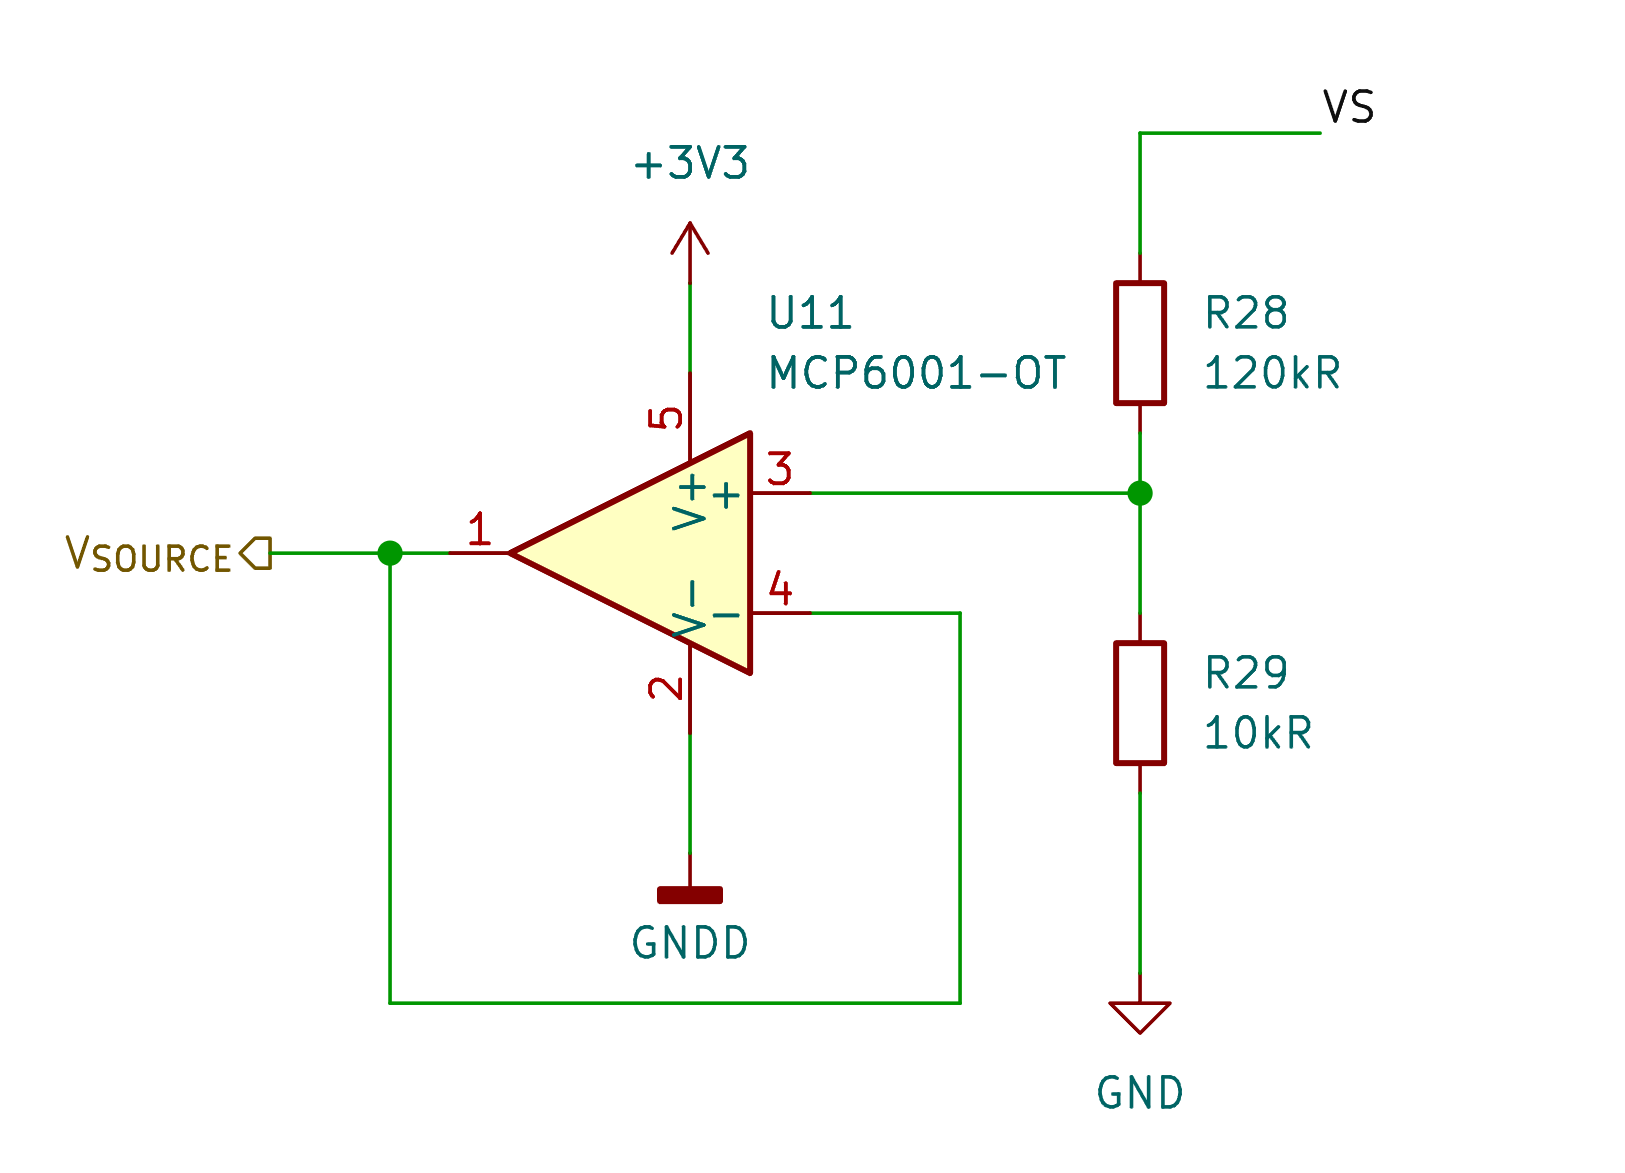
\includegraphics[width=\triplefigure]{\pics/schematics/opamp}}
        \caption{Amplifiers used in voltage and current measurements}
        \label{fig:omapms}
    \end{center}
\end{figure}

For both output voltage and current, I have applied a differential measurement method as to isolate the common-mode noise that may arise in supply switching circuits, as this can negatively impact the readings on the \gls{adc}.
In \figref{fig:getiout} the load is measured at the connections points under the resistor pads, with minimal voltage dropout as the resistance is significantly small ($10\mu \Omega$).
On the output voltage, the resistor network used in \figref{fig:getvout} is used to match the impedance across both segments, and $R1$ is used to adjust the gain of each input of the instrumentation amplifier.
For the input voltage (\figref{fig:getvin}), a sensing wire is connected at the positive terminal of the source terminal, and the value is reduced to $\approx 7.69\%$ using the voltage divider.
This same circuit is also used to measure the voltage across each arm of the bridge, in order to know the voltage at the capacitors, for nets $V_{C1}$ respectively $V_{C2}$.
Finally, each half bridge \gls{ic} contains a current sense signal $IS$ that can be utilized to either report the current flowing through the \gls{ic}, or to alert of overcurrent events.

\begin{figure}[!ht]
    \begin{center}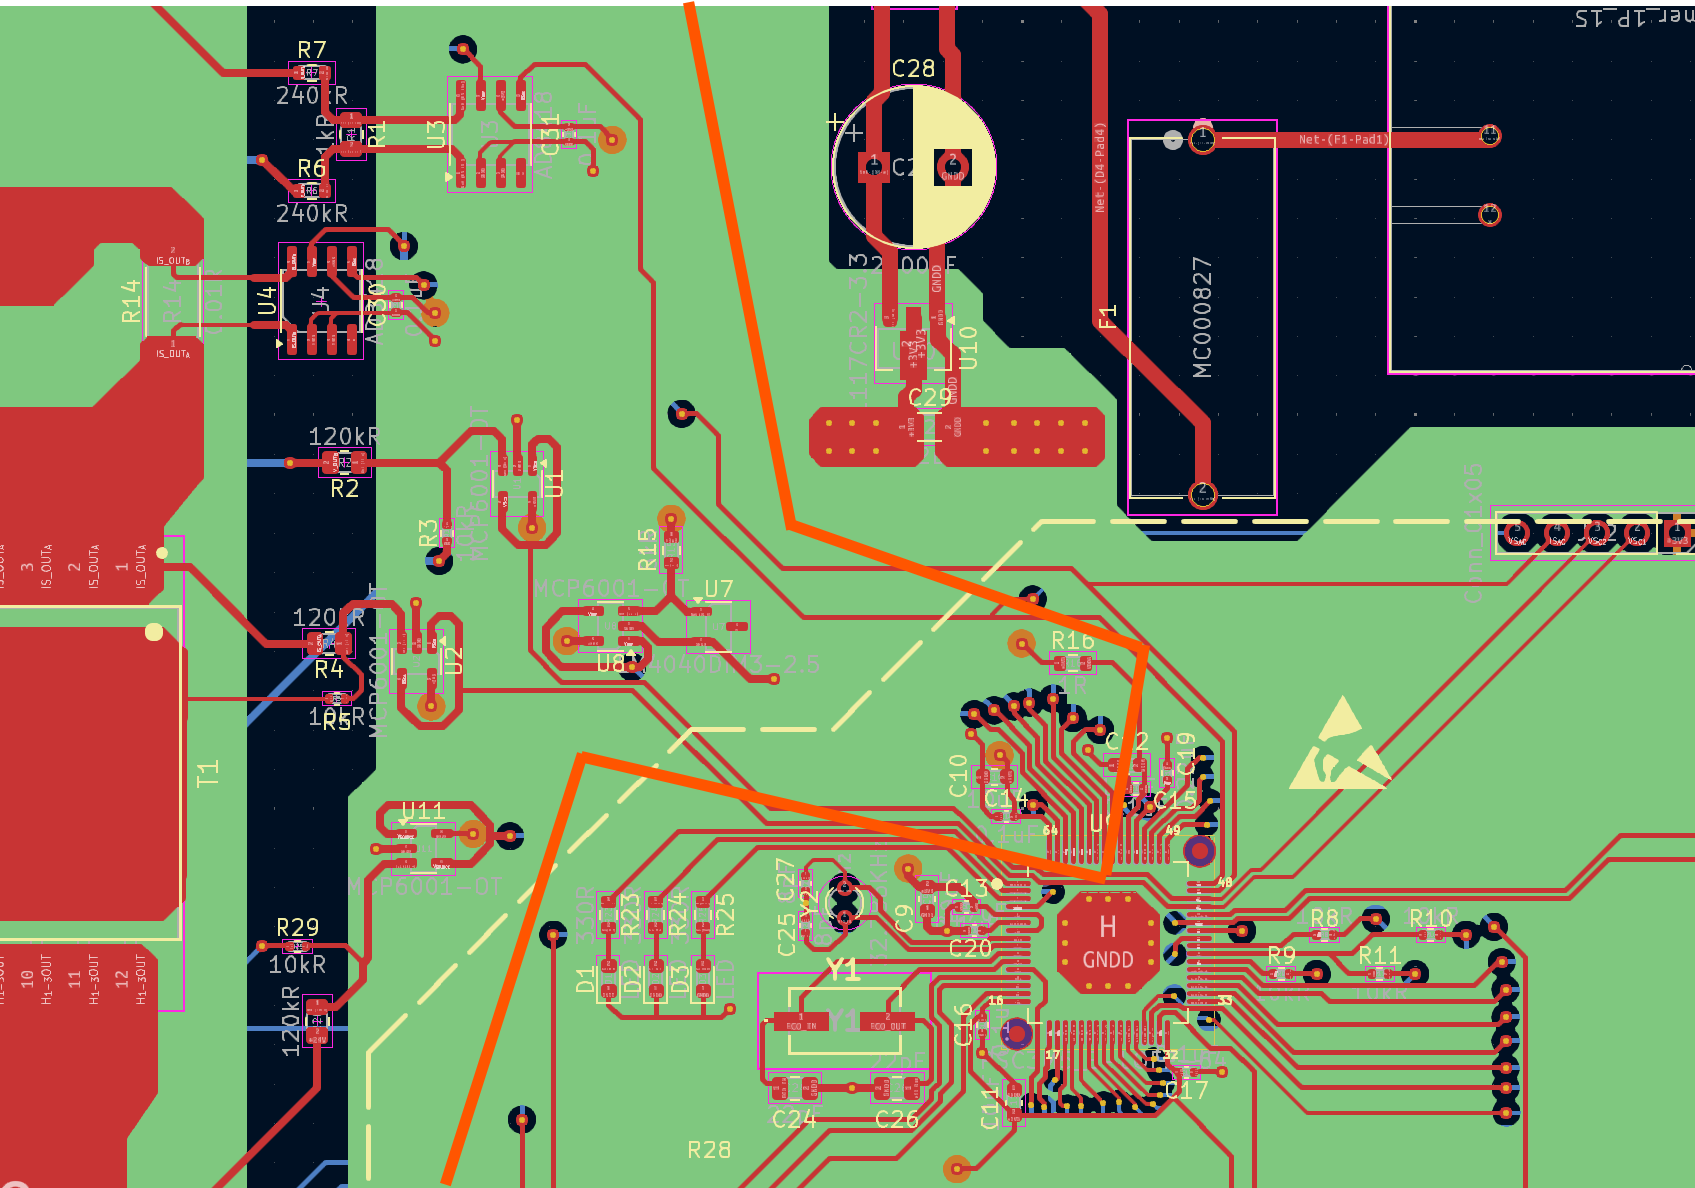
\includegraphics[width=\singlefigure]{\pics/schematics/analogzone}\end{center}
    \caption{Split by the orange line, analog signals are separated from digital wires}
    \label{fig:analogzone}
\end{figure}

Control and measurement signals used in the feedback loop have the direction of flow represented in \figref{fig:mainsch}, going to and from the \textit{MCU IO} block.
The separation in schematic is not only physical, as the number of peripherals connected to the microcontroller require space in order to be properly laid out.
These signals should be routed to accommodate for the electrical requirements in order to avoid induced noises and significant voltage drops.
Mainly, voltage and current measured are analog signals and have to pass through the \gls{adc}s, meaning that the wires should be physically as far as possible (depicted in \figref{fig:analogzone}) from any digital signals, and especially switching pulses, like the $INH$ signal\cite{zumbahlen2007basic}.
Besides control signals, other auxiliary ports are connected to the microcontroller to allow the users to implement additional functionalities depending on the application, but most importantly to create mechanisms for emergency stops or to point out the functioning state of the hardware and to upload and debug the program to be written on the microcontroller.

\begin{figure}[!ht]
    \begin{center}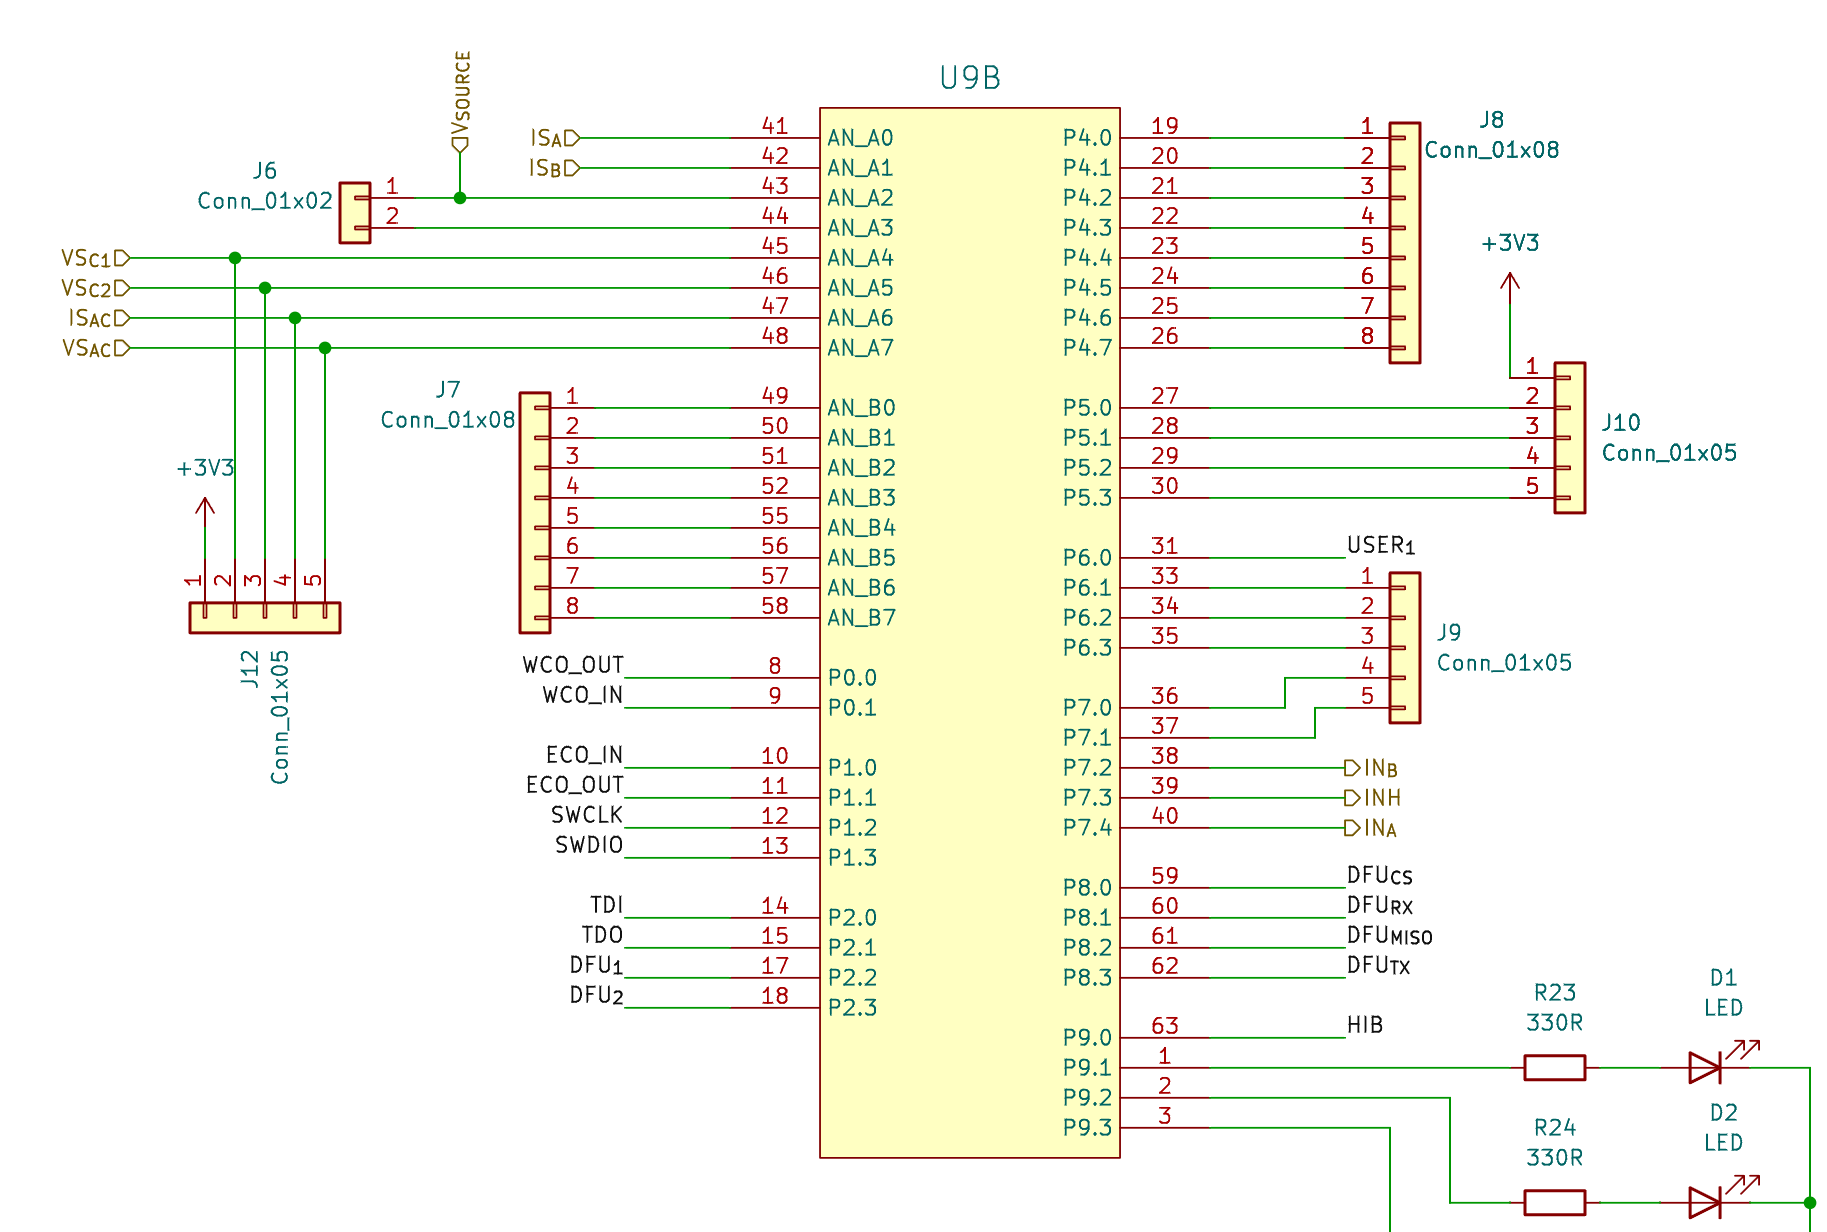
\includegraphics[width=\singlelongfigure]{\pics/schematics/mcuio}\end{center}
    \caption{Schematic representation of the I/O connections}
    \label{fig:mcuio}
\end{figure}

Even if the board already has a power input coming from the supposed photovoltaic cell, the energy provided is unreliable to supply critical areas responsible for converting the power, and besides that, another stage of voltage step-down has to be implemented in order to deliver the low voltages at which the logic circuits function at [$3.3V, 5V$].
Instead, the board has to be powered on by an individual power supply, which could give some flexibility in how the solution can draw supply rails to each \gls{ic} and can reduce the footprint on board.
There cold be multiple ways to create this architecture, but in the end, I have chosen to include a classic step-down transformer with a diode rectifier in order to power the circuit from any \gls{ac} source.
This option would ease the development of the board as energy coming from the grid is already subjected to strict control, thus requiring less components to filter the resulting input current.
For powering the components, there are 2 solutions to draw the supply rails: either have separate wires for each power domain, and in this case, separation from discrete and analogic devices, or spread the components' placement across a dedicated power plane\cite{zumbahlen2007basic}.
Since circuit requirements are not stringent, as long as current paths do not cross from one domain to another, a dedicated power plane may be sufficient for proper operation.

This leads to the final consideration of the board, deciding the stack-up of the \gls{pcb}.
Considering the previous discussion about component layout and power supplying solutions, I have decided to use a 4-layer board, each with their own signal category assignment.
\figref{fig:stack} contains a sliced representation of the board showing each layer and their attribution, matched to the color of the layer as presented in KiCad.

\begin{figure}[!ht]
    \begin{center}
        \subfloat[H-bridge section]{\label{fig:stack1}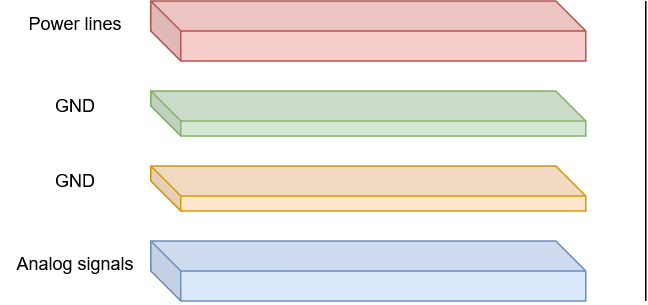
\includegraphics[width=\doublefigure]{\pics/schematics/layers2}}
        \subfloat[Logic control section]{\label{fig:stack2}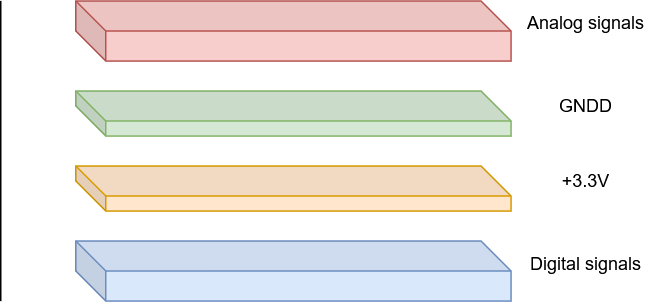
\includegraphics[width=\doublefigure]{\pics/schematics/layers1}}
        \caption{PCB stack-up}
        \label{fig:stack}
    \end{center}
\end{figure}

For \figref{fig:stack2}, the chosen order is standard in 4-layer board, made in such a way to minimize the interferences between mixed domain signals, and to decouple the analogic section from the power plane by shielding it with the ground plane.
On the power conversion section, the most important requirement is to design the traces in such a way that the board does not overheat and cause malfunction.
As suggested in both sections, outer layers have a larger cross-section than the inner layers, thus are more suitable for conducting high currents through them.
For improved thermal dissipation, maximizing the width of any trace can lead to further heat spread, and where possible, instead of using traces, copper pools can be utilized to accomplish this technique, as shown in \figref{fig:gerberbridge}.
Inner layers on this section only have shielding effect in order to reduce \gls{emi} spreading to the voltage sensing lines.

\begin{figure}[!ht]
    \begin{center}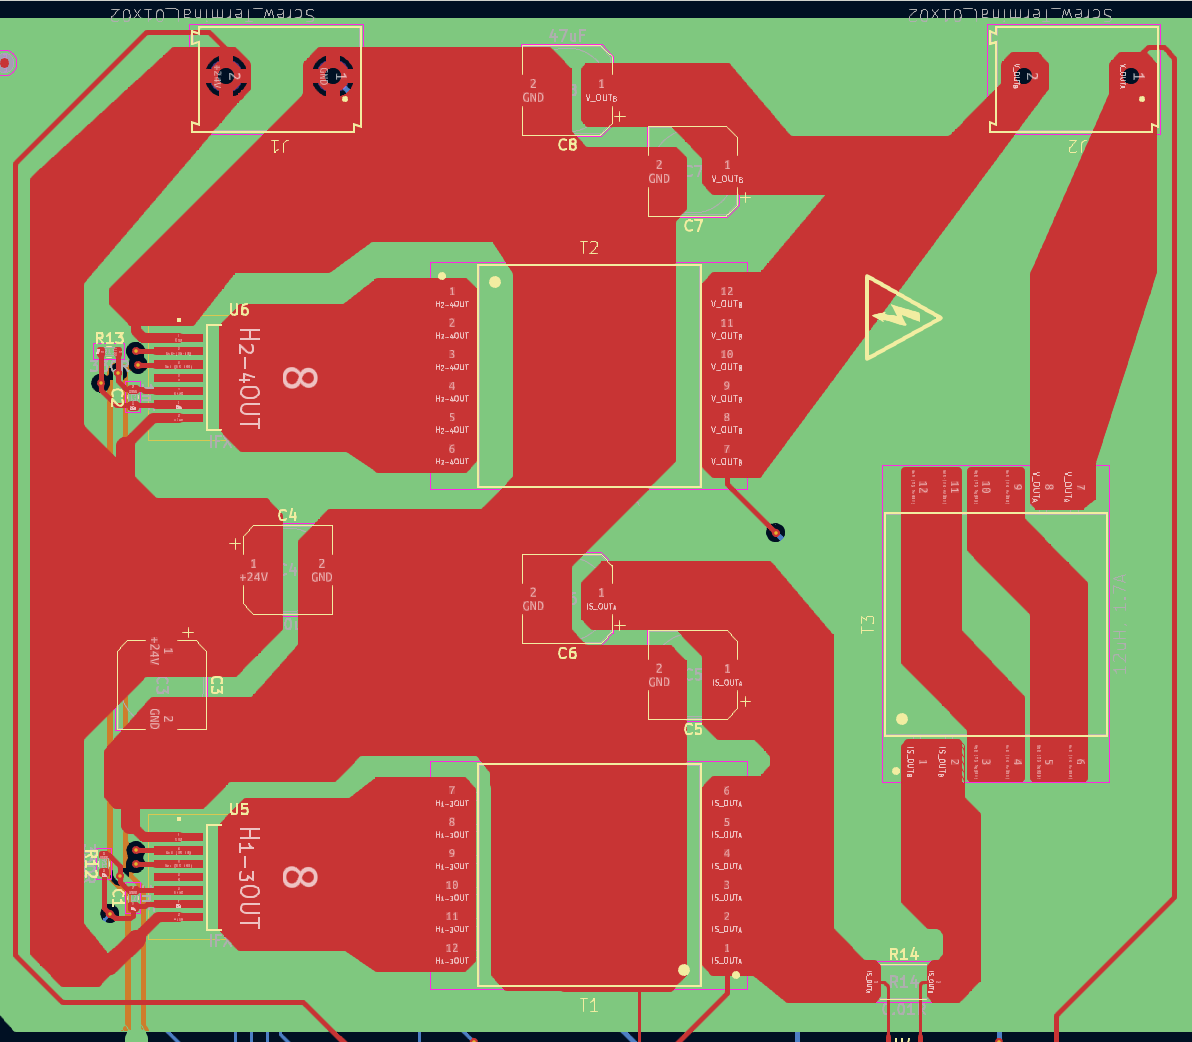
\includegraphics[width=\singlefigure]{\pics/schematics/gerberBridge}\end{center}
    \caption{Copper fill areas in red show the high voltage traces as spread out}
    \label{fig:gerberbridge}
\end{figure}

\section{Software Implementation}
\label{sec:swimp}

As expected from the previously described design, the active circuits present on the board have to be driven by the control algorithm in order for the system to properly function.
The most important component that orchestrates this aspect is the microcontroller, that hosts the peripherals necessary in order to measure both the system's parameters and to compute the \gls{pwm} duty cycle.
When talking about the software's architecture, besides the CPU that is responsible for scheduling the program and to calculate the next time period, there is a need to mention the dedicated hardware peripherals inside the microcontroller that facilitate physical to digital connections which make the solution function.
In \figref{fig:swarch} is presented how the peripherals are logically connected in order to create the control algorithm.
\begin{figure}[!ht]
    \begin{center}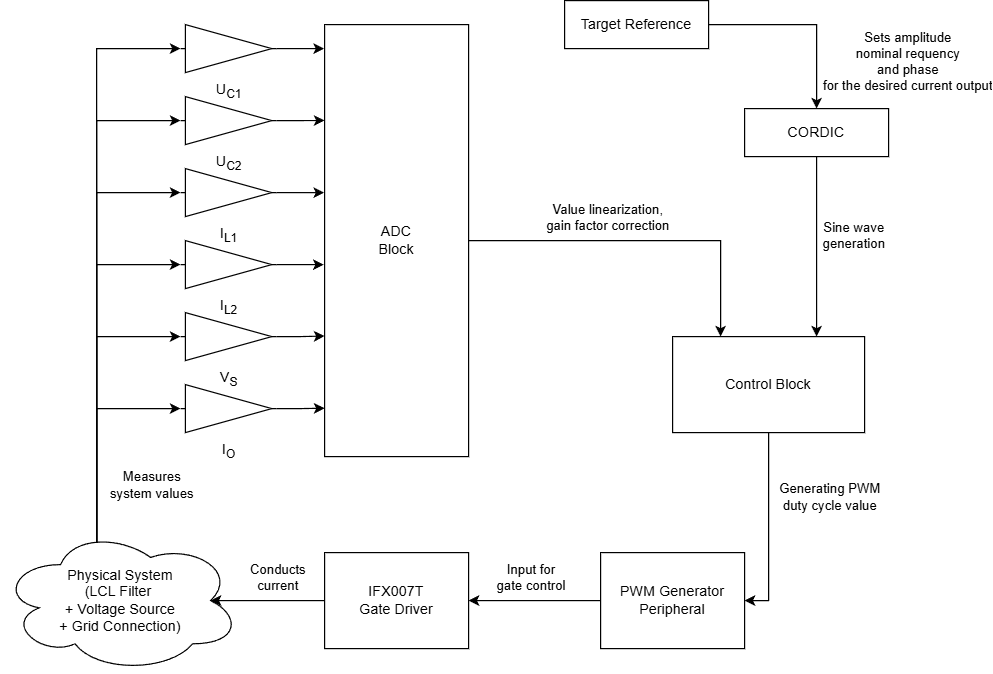
\includegraphics[width=\singlefigure]{\pics/schematics/swarch}\end{center}
    \caption{Logical representation of software architecture and peripheral usage}
    \label{fig:swarch}
\end{figure}

In layman terms, the physical circuit works in the continuous domain, meaning each current and voltage is corresponding to the analog domain.
It is not enough to only measure these, but to convert them using the \gls{adc} peripheral, which would give raw numeric values.
This block can also scale these values to floating point voltages and currents based on the PSoC3M5's documentation that implements a function call.
For the control algorithm, we need to have the output inductor's current, grid voltage, source voltage and at least one of the capacitor's voltage, since in theory, the capacitors have a complementary voltage that averages to the output source voltage.
Since the \gls{adc} peripheral can work up to 240MHz, and it takes a minimum of 4 cycles for the results, the average response time for the conversion is around $16.66\mu s$ \cite{psocdatasheet}.
If the \gls{pwm} sampling frequency is chosen as 50KHz, the \gls{pwm} counter has 1200 values, or an 11-bit resolution, which is sufficient for precise commands.
As the \gls{adc} block functions independent of the CPU, there is no need to optimize the scheduler to take each conversion into account, as once the operation is done, we can trigger the peripheral to update the measured values to the software.
The same procedure is done for computing the reference value for the desired sine wave, as we can offload the workload from the CPU to the CORDIC block.
CORDIC is a special hardware acceleration block that can compute trigonometrical functions and the square roots much faster than traditional software methods, meaning it is appropriate in this instance to update the reference sine wave every \gls{pwm} time period.
Having all of the necessary values to compute the next duty cycle, the CPU them computes the correct command that is sent to the \gls{pwm} signal generation block.
To drive the MOSFETs inside the IFX007T, there are 3 signals used as follows:
\begin{itemize}
    \item ${INH}$ is the signal driven using \gls{pwm}, that is common to both half-bridges;
    \item $IN_A$ and $IN_B$ are driven complementary; when one half-bridge drives the high-side transistor, the other should also open the low-side transistor for allowing the system to function under \gls{dcm}.
\end{itemize}
\chapter{Conclusions and Further Exploration}
\label{chap:conclusions}


\chapter{Table of Contributions}
\label{chap:contributions}

\begin{table}[ht!]
\begin{tabular}{|c|c|c|}
\hline
\multicolumn{3}{|c|}{\textbf{Discontinuous Current Conduction Mode in Solar Energy Production}} \\
\multicolumn{3}{|c|}{\textbf{Graduate: Bontaș Cezar-Octavian}} \\
\multicolumn{3}{|c|}{\textbf{Advisor: Petrescu Cătălin-Dumitru}} \\
\hline
 & Activity & Duration [days] \\
\hline
1 & Discussion with the advisor related to targets, & 1\\
& objectives, working principles & \\
\hline
2 & Gathering, reading and understanding & 7\\
& related works, articles, books & \\
\hline
3 & Working on demonstrating the analytical & 7\\
& model of the circuit's behaviour &\\
\hline
4 & Creating the Simulink model and preliminary & 5\\
& testing for debugging the model & \\
\hline
5 & Testing the Simulink model in different & 2\\
& scenarios, gathering result data & \\
\hline
6 & Selecting components for the physical prototype& 5\\
\hline
7 & Designing the PCB prototype in KiCad& 30\\
\hline
8 & Prototype assembly testing & 1\\
\hline
9 & Writing code for the prototype & 2\\
\hline
10 & Writing the thesis& 21\\
\hline
Total & & 81 \\
\hline
\end{tabular}
\centering
\caption{List of Personal Contributions}
\label{tab:contrib_list}
\end{table}

%%%%%%%%%%%%%%%%%%%%%% back matter %%%%%%%%%%%%%%%%%%%%%%%%%%%%%%%%%%%%%%
%\appendix
%\appendixpage
%\addappheadtotoc
%\begin{appendices}																				  % from here onwards are the appendices
%    \chapter{Listings}
\label{chap:codes}
%\end{appendices}

\cleardoublepage

\printbibliography[heading=bibintoc]
\end{document}